\documentclass[annual]{acmsiggraph}
%
\usepackage{graphicx}
\usepackage{pxfonts}
\usepackage{algorithm}
\usepackage{algorithmic}
\usepackage{epstopdf}
\usepackage{fullpage}
\usepackage{epic}
\usepackage{eepic}


\title{CS5625 Final Project Proposal (Revised)}

\author{Michael Flashman\thanks{e-mail:mtf53@cornell.edu}\\Cornell University \and Tianhe Zhang \thanks{e-mail:tz249@cornell.edu}\\Cornell University}

\pdfauthor{Michael Flashman, Tianhe Zhang}

\begin{document}


\maketitle


\section{Overview}
We propose a simple  game inspired by the short play \textit{Act Without Words I}, by Samuel Becket.   
The setting for the game is barren dessert.  In the middle of this dessert  stands a palm tree, and a pile of  shiny colored spheres.  The premise of the game is to launch these spheres off at some distant target by using the palm tree as an impromptu catapult.   When the player hits the target, the tree grows taller.  Additional trees may be added or removed from the scene as desired. See Fig. 1.

\begin{figure}[b]
\begin{center}
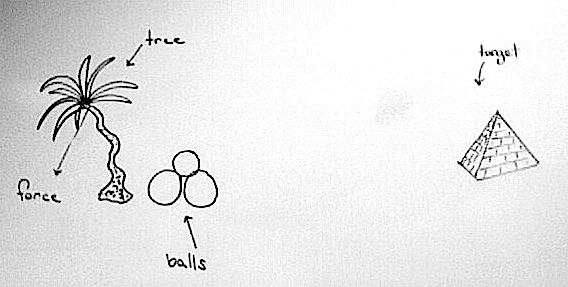
\includegraphics[height=100pt]{scene.png}
\caption{Crude sketch of game scene with a single frond--less palm tree.}
\label{default}
\end{center}
\end{figure}


\section{Technical Components}
The primary technical component of our game is the procedural generation of interactive palm trees.  We choose the palm tree for it's relatively simple organization: trunk, fronds, leaves.  But a few simple changes to model parameters yield a broad range of distinct plant species.  The generative task consists of a modeling component and a rendering component.  For the modeling component, we first generate a parametrized tree skeleton to represent the basic positioning of trunk fronds and leaves.  From the skeleton we  build custom mesh surfaces for the trunk fronds and leaves.  In general, it will suffice to use relatively simply geometry for our mesh surfaces;  much of the complexity of the tree will come from the particular skeleton configuration and texturing.   While will so not directly follow a single paper, many of the problems and solutions to modeling trees and vegetation are considered in \cite{bloomenthal1985}  \cite{kharlamov2008} \cite{sousa2008} 

The rendering component concerns texturing the mesh surfaces and adding lighting effects.  We will  explore  procedural  generation of bark textures following the methods described in \cite{elbert2002}.  The nice thing about the procedural approach, rather than say image texturing, is that we gain immediate access to normal maps/height maps / , etc.  So we are immediately in a position to implement  normal mapping technique (such as relief mapping).  Depending on the how well our generated textures look, we may also explore a texture synthesis approach, which uses use real bark image tile to create seamless and irregular surface textures \cite{ashikhmin2001}.   The main problem with approach is that a height map is no where to be seen.  Fortunately this problem may be remedied using height map reconstruction algorithms described in \cite{wang2003}.   For the leaf rendering, we will apply a simple opacity texture to capture the effect of back lighting of thin leaves.  Shadow mapping techniques and ambient occlusion from previous assignments may also be incorporated to improve overall appearance.  

A significant challenge with procedurally generated vegetation is breaking away from the organization inherent to the generative procedure.  In addition, it is important to get physically plausible positioning.  To that end, and with a broader interest in interaction,  we will perform a simple physics simulation and collision detection on the tree skeleton.   We will not try to model the physics exactly, but rather think of the tree in terms of simple mass and spring system.  Though the effect may be comical rather than realistic, the result should not be unpleasant.  As time allows we will consider different physical constant schemes to give more natural behavior in the leaves.   

Finally we will implement the game component of the project.  Aside from the basic user interface, the main technical challenge is connecting the spheres (to be catapulted)  to the palm tree in a physically plausible way.  This requires that we add the sphere to our physics engine and perform collision detection.    We will incorporate some basic visual feedback when our spheres hit something, such as adding large colored spots or holes. When the sphere hits the target, we will grow the main palm tree or grow a new palm tree depending on the number of times the target is hit.

Above is our main goal for this project. However, if we have more time, we will consider some of the extensions described below:
\begin{enumerate}
\item{Apply procedural wind animation to the tree  \cite{renaldas2008}  }
\item{Create non planer terrain using sand dune model \cite{momiji2002}}
\item{Apply level of detail to tree mesh and textures and/or terrain}
\item{Implement full day scenario such that the sun and the sky change overtime.}
\end{enumerate}

%\begin{enumerate}
\section{Tentative Schedule}
\begin{itemize}
\item{Week 1: April 1 - April 7}

\begin{enumerate}
\item{Talk to Prof. Bala and the TAs about our idea. - Michael and Tianhe }
\item{Finalize our idea and proposal. - Michael and Tianhe}
\item{Have a clear idea about how we want to implement our tree model. This includes discussion about all the features we might want so that we can make it generic. - Michael and Tianhe}
\item{Get familiar with the framework of the base code so that we are ready to implement. - Michael and Tianhe}
\end{enumerate}

\item{Week 2: April 8 - April 14}

\begin{enumerate}
\item{Implement physics engine and particle edge collision detection. - Michael and Tianhe}
\item{Tree model: build the trunk model procedurally . - Tianhe}
\end{enumerate}

\item{Week 3: April 15 - April 21}

\begin{enumerate}
\item{Tree model: build the fronds model procedurally. - Michael}
\item{Testing this physically interactive mesh. - Michael and Tianhe}

\end{enumerate}

\item{Week 4: April 22 - April 28}

\begin{enumerate}
\item{Learn how to procedurally generate texture for barks. - Michael}
\item{Implement the texture mapping for the bark and leaves. -Tianhe}
\end{enumerate}

\item{Week 5: April 29 - May 5}

\begin{enumerate}
\item{Implementation of normal mapping for the barks. -Tianhe }
\item{Implementation for the game related stuff. - Michael}

\end{enumerate}

\item{Week 6: May 5 - May 11}

\begin{enumerate}
\item{Wrap up - Michael and Tianhe}
\item{Implement some of the extension if have time - Michael and Tianhe}
\item{Test and report - Michael and Tianhe}
\end{enumerate}

\item{Week 6: May 12 - May 15}

\begin{enumerate}
\item{Implement some of the extension if have time - Michael and Tianhe}
\item{Test and report - Michael and Tianhe}
\end{enumerate}

\end{itemize}


\bibliographystyle{acmsiggraph}
\bibliography{bibliography}



\end{document}
